\documentclass[]{book}
\usepackage{lmodern}
\usepackage{amssymb,amsmath}
\usepackage{ifxetex,ifluatex}
\usepackage{fixltx2e} % provides \textsubscript
\ifnum 0\ifxetex 1\fi\ifluatex 1\fi=0 % if pdftex
  \usepackage[T1]{fontenc}
  \usepackage[utf8]{inputenc}
\else % if luatex or xelatex
  \ifxetex
    \usepackage{mathspec}
  \else
    \usepackage{fontspec}
  \fi
  \defaultfontfeatures{Ligatures=TeX,Scale=MatchLowercase}
\fi
% use upquote if available, for straight quotes in verbatim environments
\IfFileExists{upquote.sty}{\usepackage{upquote}}{}
% use microtype if available
\IfFileExists{microtype.sty}{%
\usepackage{microtype}
\UseMicrotypeSet[protrusion]{basicmath} % disable protrusion for tt fonts
}{}
\usepackage[margin=1in]{geometry}
\usepackage{hyperref}
\hypersetup{unicode=true,
            pdftitle={e.GO Digital Hackathon},
            pdfauthor={Team: Hugs for bugs},
            pdfborder={0 0 0},
            breaklinks=true}
\urlstyle{same}  % don't use monospace font for urls
\usepackage{natbib}
\bibliographystyle{plainnat}
\usepackage{color}
\usepackage{fancyvrb}
\newcommand{\VerbBar}{|}
\newcommand{\VERB}{\Verb[commandchars=\\\{\}]}
\DefineVerbatimEnvironment{Highlighting}{Verbatim}{commandchars=\\\{\}}
% Add ',fontsize=\small' for more characters per line
\usepackage{framed}
\definecolor{shadecolor}{RGB}{248,248,248}
\newenvironment{Shaded}{\begin{snugshade}}{\end{snugshade}}
\newcommand{\AlertTok}[1]{\textcolor[rgb]{0.94,0.16,0.16}{#1}}
\newcommand{\AnnotationTok}[1]{\textcolor[rgb]{0.56,0.35,0.01}{\textbf{\textit{#1}}}}
\newcommand{\AttributeTok}[1]{\textcolor[rgb]{0.77,0.63,0.00}{#1}}
\newcommand{\BaseNTok}[1]{\textcolor[rgb]{0.00,0.00,0.81}{#1}}
\newcommand{\BuiltInTok}[1]{#1}
\newcommand{\CharTok}[1]{\textcolor[rgb]{0.31,0.60,0.02}{#1}}
\newcommand{\CommentTok}[1]{\textcolor[rgb]{0.56,0.35,0.01}{\textit{#1}}}
\newcommand{\CommentVarTok}[1]{\textcolor[rgb]{0.56,0.35,0.01}{\textbf{\textit{#1}}}}
\newcommand{\ConstantTok}[1]{\textcolor[rgb]{0.00,0.00,0.00}{#1}}
\newcommand{\ControlFlowTok}[1]{\textcolor[rgb]{0.13,0.29,0.53}{\textbf{#1}}}
\newcommand{\DataTypeTok}[1]{\textcolor[rgb]{0.13,0.29,0.53}{#1}}
\newcommand{\DecValTok}[1]{\textcolor[rgb]{0.00,0.00,0.81}{#1}}
\newcommand{\DocumentationTok}[1]{\textcolor[rgb]{0.56,0.35,0.01}{\textbf{\textit{#1}}}}
\newcommand{\ErrorTok}[1]{\textcolor[rgb]{0.64,0.00,0.00}{\textbf{#1}}}
\newcommand{\ExtensionTok}[1]{#1}
\newcommand{\FloatTok}[1]{\textcolor[rgb]{0.00,0.00,0.81}{#1}}
\newcommand{\FunctionTok}[1]{\textcolor[rgb]{0.00,0.00,0.00}{#1}}
\newcommand{\ImportTok}[1]{#1}
\newcommand{\InformationTok}[1]{\textcolor[rgb]{0.56,0.35,0.01}{\textbf{\textit{#1}}}}
\newcommand{\KeywordTok}[1]{\textcolor[rgb]{0.13,0.29,0.53}{\textbf{#1}}}
\newcommand{\NormalTok}[1]{#1}
\newcommand{\OperatorTok}[1]{\textcolor[rgb]{0.81,0.36,0.00}{\textbf{#1}}}
\newcommand{\OtherTok}[1]{\textcolor[rgb]{0.56,0.35,0.01}{#1}}
\newcommand{\PreprocessorTok}[1]{\textcolor[rgb]{0.56,0.35,0.01}{\textit{#1}}}
\newcommand{\RegionMarkerTok}[1]{#1}
\newcommand{\SpecialCharTok}[1]{\textcolor[rgb]{0.00,0.00,0.00}{#1}}
\newcommand{\SpecialStringTok}[1]{\textcolor[rgb]{0.31,0.60,0.02}{#1}}
\newcommand{\StringTok}[1]{\textcolor[rgb]{0.31,0.60,0.02}{#1}}
\newcommand{\VariableTok}[1]{\textcolor[rgb]{0.00,0.00,0.00}{#1}}
\newcommand{\VerbatimStringTok}[1]{\textcolor[rgb]{0.31,0.60,0.02}{#1}}
\newcommand{\WarningTok}[1]{\textcolor[rgb]{0.56,0.35,0.01}{\textbf{\textit{#1}}}}
\usepackage{longtable,booktabs}
\usepackage{graphicx,grffile}
\makeatletter
\def\maxwidth{\ifdim\Gin@nat@width>\linewidth\linewidth\else\Gin@nat@width\fi}
\def\maxheight{\ifdim\Gin@nat@height>\textheight\textheight\else\Gin@nat@height\fi}
\makeatother
% Scale images if necessary, so that they will not overflow the page
% margins by default, and it is still possible to overwrite the defaults
% using explicit options in \includegraphics[width, height, ...]{}
\setkeys{Gin}{width=\maxwidth,height=\maxheight,keepaspectratio}
\IfFileExists{parskip.sty}{%
\usepackage{parskip}
}{% else
\setlength{\parindent}{0pt}
\setlength{\parskip}{6pt plus 2pt minus 1pt}
}
\setlength{\emergencystretch}{3em}  % prevent overfull lines
\providecommand{\tightlist}{%
  \setlength{\itemsep}{0pt}\setlength{\parskip}{0pt}}
\setcounter{secnumdepth}{5}
% Redefines (sub)paragraphs to behave more like sections
\ifx\paragraph\undefined\else
\let\oldparagraph\paragraph
\renewcommand{\paragraph}[1]{\oldparagraph{#1}\mbox{}}
\fi
\ifx\subparagraph\undefined\else
\let\oldsubparagraph\subparagraph
\renewcommand{\subparagraph}[1]{\oldsubparagraph{#1}\mbox{}}
\fi

%%% Use protect on footnotes to avoid problems with footnotes in titles
\let\rmarkdownfootnote\footnote%
\def\footnote{\protect\rmarkdownfootnote}

%%% Change title format to be more compact
\usepackage{titling}

% Create subtitle command for use in maketitle
\providecommand{\subtitle}[1]{
  \posttitle{
    \begin{center}\large#1\end{center}
    }
}

\setlength{\droptitle}{-2em}

  \title{e.GO Digital Hackathon}
    \pretitle{\vspace{\droptitle}\centering\huge}
  \posttitle{\par}
    \author{Team: Hugs for bugs}
    \preauthor{\centering\large\emph}
  \postauthor{\par}
      \predate{\centering\large\emph}
  \postdate{\par}
    \date{2019-05-24}

\usepackage{booktabs}

\begin{document}
\maketitle

{
\setcounter{tocdepth}{1}
\tableofcontents
}
\hypertarget{task}{%
\chapter{Task}\label{task}}

The e.GO life is generating, collecting and processing serveral data per second. Those data could be very valuable for us. Especially when you think of developing new innovative business models. Your task is to develop value-adding services for the e.GO Life and its user considering the provided data.

\hypertarget{value-adding-services}{%
\chapter{Value-adding services}\label{value-adding-services}}

Our services should support at least the following functions:

\begin{itemize}
\tightlist
\item
  Intelligently choose the parking lot

  \begin{itemize}
  \tightlist
  \item
    location convenient
  \item
    cheap price
  \item
    support egoPay
  \end{itemize}
\item
  Shortly reservation for the parking lot

  \begin{itemize}
  \tightlist
  \item
    estimating the arrival time
  \item
    automatically reserve the parking space in advance
  \item
    message notification
  \end{itemize}
\item
  Immediately payment -- egoPay

  \begin{itemize}
  \tightlist
  \item
    no worry about parking time
  \item
    automatic charging fees while leaving
  \end{itemize}
\item
  Ego drive-thru

  \begin{itemize}
  \tightlist
  \item
    food reservation from supermarket
  \item
    food pick up from parking lot
  \item
    food payment by egoPay
  \end{itemize}
\end{itemize}

\hypertarget{dataset-overview}{%
\chapter{Dataset Overview}\label{dataset-overview}}

\hypertarget{we-prepare-a-dataset-as-shown-below}{%
\section{We prepare a dataset, as shown below}\label{we-prepare-a-dataset-as-shown-below}}

\begin{Shaded}
\begin{Highlighting}[]
\ImportTok{import}\NormalTok{ pandas }\ImportTok{as}\NormalTok{ pd}
\NormalTok{df }\OperatorTok{=}\NormalTok{ pd.read_csv(}\StringTok{'location.csv'}\NormalTok{, sep}\OperatorTok{=}\StringTok{'}\CharTok{\textbackslash{}t}\StringTok{'}\NormalTok{, index_col}\OperatorTok{=}\DecValTok{0}\NormalTok{)}
\NormalTok{df}
\end{Highlighting}
\end{Shaded}

\begin{verbatim}
##   location_name   latitude  longitude  price/hour  is_outdoor  ego_pay
## 0          e.Go  50.781624   6.046581           2           1        1
## 1       Super C  50.778430   6.078702           3           1        0
## 2        Bushof  50.777557   6.090270           4           1        0
## 3  Hauptbahnhof  50.767911   6.091582           4           0        1
## 4    Euregiozoo  50.763672   6.115565           3           1        1
\end{verbatim}

\begin{itemize}
\tightlist
\item
  location\_name: the parking plot location
\item
  latitude: latitude of the parking plot
\item
  longtitude: longtitude of the parking plot
\item
  price/hour: price to be charged per hour
\item
  is\_outdoor: is the parking plot outdoor or inside
\item
  ego\_pay: does the parking plot support ``EgoPay''
\end{itemize}

\hypertarget{get-current-location-update-location}{%
\section{Get current location, update location}\label{get-current-location-update-location}}

\begin{Shaded}
\begin{Highlighting}[]
\ImportTok{import}\NormalTok{ requests}
\KeywordTok{class}\NormalTok{ EgoCar:}
    
    \KeywordTok{def} \FunctionTok{__init__}\NormalTok{(}\VariableTok{self}\NormalTok{, api_url):}
        \VariableTok{self}\NormalTok{.api_url }\OperatorTok{=}\NormalTok{ api_url}
        \VariableTok{self}\NormalTok{.api_key }\OperatorTok{=} \StringTok{'7443363c-4304-4c56-9df0-6af4af40c613'}
        \VariableTok{self}\NormalTok{.header }\OperatorTok{=}\NormalTok{ \{}\StringTok{'Content-type'}\NormalTok{: }\StringTok{'application/json'}\NormalTok{, }\StringTok{'X-Api-Key'}\NormalTok{: }\VariableTok{self}\NormalTok{.api_key\}}
        
    \KeywordTok{def}\NormalTok{ get_location(}\VariableTok{self}\NormalTok{):}
\NormalTok{        res }\OperatorTok{=}\NormalTok{ requests.get(}\VariableTok{self}\NormalTok{.api_url, headers}\OperatorTok{=}\VariableTok{self}\NormalTok{.header)}
\NormalTok{        location }\OperatorTok{=}\NormalTok{ res.json()[}\StringTok{'location'}\NormalTok{]}
        \ControlFlowTok{return}\NormalTok{ location}
    
    \KeywordTok{def}\NormalTok{ update_location(}\VariableTok{self}\NormalTok{, new_location):}
\NormalTok{        x, y }\OperatorTok{=}\NormalTok{ new_location.split(}\StringTok{','}\NormalTok{)}
\NormalTok{        x, y }\OperatorTok{=} \BuiltInTok{float}\NormalTok{(x), }\BuiltInTok{float}\NormalTok{(y)}
        \ControlFlowTok{if}\NormalTok{ x }\OperatorTok{>=} \DecValTok{-90} \KeywordTok{and}\NormalTok{ x }\OperatorTok{<=} \DecValTok{90} \KeywordTok{and}\NormalTok{ y }\OperatorTok{>=} \DecValTok{-90} \KeywordTok{and}\NormalTok{ y }\OperatorTok{<=} \DecValTok{90}\NormalTok{:}
\NormalTok{            data }\OperatorTok{=}\NormalTok{ \{}\StringTok{'location'}\NormalTok{: new_location\}}
\NormalTok{            requests.patch(}\VariableTok{self}\NormalTok{.api_url, json}\OperatorTok{=}\NormalTok{data, headers}\OperatorTok{=}\VariableTok{self}\NormalTok{.header)}
            \BuiltInTok{print}\NormalTok{(}\StringTok{'new location: '}\NormalTok{, new_location)}
        \ControlFlowTok{else}\NormalTok{:}
            \BuiltInTok{print}\NormalTok{(}\StringTok{'[Error] Latitude value must be between -90 and 90'}\NormalTok{)}
\end{Highlighting}
\end{Shaded}

\begin{itemize}
\tightlist
\item
  get current location
\end{itemize}

\begin{Shaded}
\begin{Highlighting}[]
\NormalTok{api_url }\OperatorTok{=} \StringTok{'https://ego-vehicle-api.azurewebsites.net/api/v1/vehicle/signals'}
\NormalTok{ego_car }\OperatorTok{=}\NormalTok{ EgoCar(api_url)}
\BuiltInTok{print}\NormalTok{(}\StringTok{'current location: '}\NormalTok{, ego_car.get_location())}
\end{Highlighting}
\end{Shaded}

\begin{verbatim}
## current location:  50.00, 6.00
\end{verbatim}

\begin{itemize}
\tightlist
\item
  update location
\end{itemize}

\begin{Shaded}
\begin{Highlighting}[]
\NormalTok{ego_car.update_location(}\StringTok{'50.00, 6.00'}\NormalTok{)}
\end{Highlighting}
\end{Shaded}

\begin{verbatim}
## new location:  50.00, 6.00
\end{verbatim}

\hypertarget{intelligent-choose-parking-lot}{%
\chapter{Intelligent choose parking lot}\label{intelligent-choose-parking-lot}}

Intelligent, we mean that we should use smart algorithms to choose the most appropriate parking lot, considering the distance, price and etc.

\begin{itemize}
\tightlist
\item
  Calculate Geographical distance
\end{itemize}

\begin{Shaded}
\begin{Highlighting}[]
\ImportTok{from}\NormalTok{ geopy.distance }\ImportTok{import}\NormalTok{ geodesic}
\ImportTok{from}\NormalTok{ geopy.geocoders }\ImportTok{import}\NormalTok{ Nominatim}
\KeywordTok{class}\NormalTok{ GeoDistance:}
    
    \KeywordTok{def} \FunctionTok{__init__}\NormalTok{(}\VariableTok{self}\NormalTok{):}
        \VariableTok{self}\NormalTok{.geolocator }\OperatorTok{=}\NormalTok{ Nominatim(user_agent}\OperatorTok{=}\StringTok{"demo"}\NormalTok{)}
        
    \KeywordTok{def}\NormalTok{ get_geo_position(}\VariableTok{self}\NormalTok{, location):}
\NormalTok{        addr }\OperatorTok{=} \VariableTok{self}\NormalTok{.geolocator.geocode(location)}
        \ControlFlowTok{return}\NormalTok{ (addr.latitude, addr.longitude)}
    
    \KeywordTok{def}\NormalTok{ get_location(}\VariableTok{self}\NormalTok{, geo_position):}
\NormalTok{        location }\OperatorTok{=} \VariableTok{self}\NormalTok{.geolocator.reverse(geo_position)}
        \ControlFlowTok{try}\NormalTok{:}
\NormalTok{            addr }\OperatorTok{=}\NormalTok{ location.raw[}\StringTok{'address'}\NormalTok{]}
            \ControlFlowTok{return} \StringTok{'}\SpecialCharTok{\{road\}}\StringTok{, }\SpecialCharTok{\{city_district\}}\StringTok{, }\SpecialCharTok{\{city\}}\StringTok{, }\SpecialCharTok{\{postcode\}}\StringTok{'}\NormalTok{.}\BuiltInTok{format}\NormalTok{(}\OperatorTok{**}\NormalTok{addr)}
        \ControlFlowTok{except}\NormalTok{:}
            \ControlFlowTok{return}\NormalTok{ location.address}
            
    \KeywordTok{def}\NormalTok{ calc_geo_distance(}\VariableTok{self}\NormalTok{, origin, destination):}
\NormalTok{        distance }\OperatorTok{=}\NormalTok{ geodesic(origin, destination).km}
        \ControlFlowTok{return}\NormalTok{ distance}
        
\end{Highlighting}
\end{Shaded}

\begin{itemize}
\tightlist
\item
  First get the current location
\end{itemize}

\begin{Shaded}
\begin{Highlighting}[]
\NormalTok{api_url }\OperatorTok{=} \StringTok{'https://ego-vehicle-api.azurewebsites.net/api/v1/vehicle/signals'}
\NormalTok{ego_car }\OperatorTok{=}\NormalTok{ EgoCar(api_url)}
\NormalTok{curr_loc }\OperatorTok{=}\NormalTok{ ego_car.get_location()}
\BuiltInTok{print}\NormalTok{(}\StringTok{'current location: '}\NormalTok{, curr_loc)}
\end{Highlighting}
\end{Shaded}

\begin{verbatim}
## current location:  50.00, 6.00
\end{verbatim}

\begin{Shaded}
\begin{Highlighting}[]
\NormalTok{geo_dis }\OperatorTok{=}\NormalTok{ GeoDistance()}
\NormalTok{addr }\OperatorTok{=}\NormalTok{ geo_dis.get_location(curr_loc)}
\BuiltInTok{print}\NormalTok{(}\StringTok{'current address: '}\NormalTok{, addr)}
\end{Highlighting}
\end{Shaded}

\begin{verbatim}
## current address:  Kiischpelt, Canton Wiltz, 9776, Lëtzebuerg
\end{verbatim}

\begin{itemize}
\tightlist
\item
  Calculate distance to parking lot
\end{itemize}

\begin{Shaded}
\begin{Highlighting}[]
\NormalTok{pd.options.mode.chained_assignment }\OperatorTok{=} \VariableTok{None}
\NormalTok{df_dis }\OperatorTok{=}\NormalTok{ df[[}\StringTok{'location_name'}\NormalTok{, }\StringTok{'latitude'}\NormalTok{, }\StringTok{'longitude'}\NormalTok{]]}
\NormalTok{origin }\OperatorTok{=}\NormalTok{ ego_car.get_location()}
\NormalTok{destination }\OperatorTok{=} \BuiltInTok{zip}\NormalTok{(df_dis[}\StringTok{'latitude'}\NormalTok{].values, df_dis[}\StringTok{'longitude'}\NormalTok{].values)}
\NormalTok{df_dis[}\StringTok{'distance/km'}\NormalTok{] }\OperatorTok{=}\NormalTok{ [geo_dis.calc_geo_distance(origin, des) }\ControlFlowTok{for}\NormalTok{ des }\KeywordTok{in}\NormalTok{ destination]}
\NormalTok{df_dis.sort_values(}\StringTok{'distance/km'}\NormalTok{, ascending}\OperatorTok{=}\VariableTok{True}\NormalTok{)}
\end{Highlighting}
\end{Shaded}

\begin{verbatim}
##   location_name   latitude  longitude  distance/km
## 4    Euregiozoo  50.763672   6.115565    85.344859
## 3  Hauptbahnhof  50.767911   6.091582    85.667684
## 2        Bushof  50.777557   6.090270    86.730648
## 1       Super C  50.778430   6.078702    86.770605
## 0          e.Go  50.781624   6.046581    87.008247
\end{verbatim}

\begin{itemize}
\tightlist
\item
  Smart choice (toy example, with different weight on attributes)

  \begin{itemize}
  \tightlist
  \item
    distance: 0.5
  \item
    price: 0.2
  \item
    is\_outdoor: 0.1
  \item
    egoPay: 0.2
  \end{itemize}
\end{itemize}

\begin{Shaded}
\begin{Highlighting}[]
\ImportTok{from}\NormalTok{ sklearn.preprocessing }\ImportTok{import}\NormalTok{ MinMaxScaler}
\NormalTok{scaler }\OperatorTok{=}\NormalTok{ MinMaxScaler()}

\NormalTok{df_new }\OperatorTok{=}\NormalTok{ df[[}\StringTok{'price/hour'}\NormalTok{, }\StringTok{'is_outdoor'}\NormalTok{, }\StringTok{'ego_pay'}\NormalTok{]]}
\NormalTok{df_new[}\StringTok{'is_outdoor'}\NormalTok{] }\OperatorTok{=}\NormalTok{ df_new[}\StringTok{'is_outdoor'}\NormalTok{].}\BuiltInTok{apply}\NormalTok{(}\KeywordTok{lambda}\NormalTok{ x : x }\OperatorTok{^} \DecValTok{1}\NormalTok{)}
\NormalTok{df_new[}\StringTok{'ego_pay'}\NormalTok{] }\OperatorTok{=}\NormalTok{ df_new[}\StringTok{'ego_pay'}\NormalTok{].}\BuiltInTok{apply}\NormalTok{(}\KeywordTok{lambda}\NormalTok{ x : x }\OperatorTok{^} \DecValTok{1}\NormalTok{)}
\NormalTok{df_weight }\OperatorTok{=}\NormalTok{ df_new.join(df_dis[}\StringTok{'distance/km'}\NormalTok{], how}\OperatorTok{=}\StringTok{'inner'}\NormalTok{)}
\CommentTok{# max-min scaler}
\NormalTok{norm_values }\OperatorTok{=}\NormalTok{ scaler.fit_transform(df_weight.values)}
\NormalTok{norm_values}
\end{Highlighting}
\end{Shaded}

\begin{verbatim}
## array([[0.        , 0.        , 0.        , 1.        ],
##        [0.5       , 0.        , 1.        , 0.85713399],
##        [1.        , 0.        , 1.        , 0.83311221],
##        [1.        , 1.        , 0.        , 0.19407646],
##        [0.5       , 0.        , 0.        , 0.        ]])
\end{verbatim}

\begin{itemize}
\tightlist
\item
  the smaller value, the better choice
\end{itemize}

\begin{Shaded}
\begin{Highlighting}[]
\ImportTok{import}\NormalTok{ numpy }\ImportTok{as}\NormalTok{ np}
\NormalTok{cost }\OperatorTok{=}\NormalTok{ np.}\BuiltInTok{sum}\NormalTok{(norm_values }\OperatorTok{*}\NormalTok{ [}\FloatTok{0.2}\NormalTok{, }\FloatTok{0.1}\NormalTok{, }\FloatTok{0.2}\NormalTok{, }\FloatTok{0.5}\NormalTok{], axis}\OperatorTok{=}\DecValTok{1}\NormalTok{)}
\NormalTok{df_weight[}\StringTok{'cost'}\NormalTok{] }\OperatorTok{=}\NormalTok{ cost.T}
\NormalTok{df_weight.sort_values(}\StringTok{'cost'}\NormalTok{, ascending}\OperatorTok{=}\VariableTok{True}\NormalTok{)}
\end{Highlighting}
\end{Shaded}

\begin{verbatim}
##    price/hour  is_outdoor  ego_pay  distance/km      cost
## 4           3           0        0    85.344859  0.100000
## 3           4           1        0    85.667684  0.397038
## 0           2           0        0    87.008247  0.500000
## 1           3           0        1    86.770605  0.728567
## 2           4           0        1    86.730648  0.816556
\end{verbatim}

It seems the best choice is \textbf{Euregiozoo}

\hypertarget{google-map-visulization}{%
\chapter{Google Map Visulization}\label{google-map-visulization}}

\begin{itemize}
\tightlist
\item
  Code to add marker and direction
\end{itemize}

\begin{Shaded}
\begin{Highlighting}[]
\KeywordTok{class}\NormalTok{ GeoMaps:}
    
    \KeywordTok{def} \FunctionTok{__init__}\NormalTok{(}\VariableTok{self}\NormalTok{, curr_location):}
        \VariableTok{self}\NormalTok{.key }\OperatorTok{=} \StringTok{'GoogleAPIKey'}
\NormalTok{        gmaps.configure(api_key}\OperatorTok{=}\VariableTok{self}\NormalTok{.key)}
        \VariableTok{self}\NormalTok{.curr_location }\OperatorTok{=}\NormalTok{ curr_location}
        \VariableTok{self}\NormalTok{.fig }\OperatorTok{=}\NormalTok{ gmaps.figure(center}\OperatorTok{=}\VariableTok{self}\NormalTok{.curr_location, zoom_level}\OperatorTok{=}\DecValTok{12}\NormalTok{)}
        
    \KeywordTok{def}\NormalTok{ add_marker(}\VariableTok{self}\NormalTok{, marker_pos):}
\NormalTok{        markers }\OperatorTok{=}\NormalTok{ gmaps.marker_layer(marker_pos)}
        \VariableTok{self}\NormalTok{.fig.add_layer(markers)}
        \ControlFlowTok{return} \VariableTok{self}\NormalTok{.fig}
    
    \KeywordTok{def}\NormalTok{ add_direction(}\VariableTok{self}\NormalTok{, origin, destination):}
\NormalTok{        to_destination }\OperatorTok{=}\NormalTok{ gmaps.directions_layer(origin, destination)}
        \VariableTok{self}\NormalTok{.fig.add_layer(to_destination)}
        \ControlFlowTok{return} \VariableTok{self}\NormalTok{.fig}
    
    \KeywordTok{def}\NormalTok{ get_curr_location(}\VariableTok{self}\NormalTok{):}
        \ControlFlowTok{return} \VariableTok{self}\NormalTok{.curr_location}
    
    \KeywordTok{def}\NormalTok{ update_location(}\VariableTok{self}\NormalTok{, new_location):}
        \VariableTok{self}\NormalTok{.curr_location }\OperatorTok{=}\NormalTok{ new_location}
\end{Highlighting}
\end{Shaded}

\begin{itemize}
\tightlist
\item
  Mark current location
\end{itemize}

\begin{Shaded}
\begin{Highlighting}[]
\NormalTok{knitr}\OperatorTok{::}\KeywordTok{include_graphics}\NormalTok{(}\StringTok{"img/google_marker.png"}\NormalTok{)}
\end{Highlighting}
\end{Shaded}

\begin{figure}

{\centering 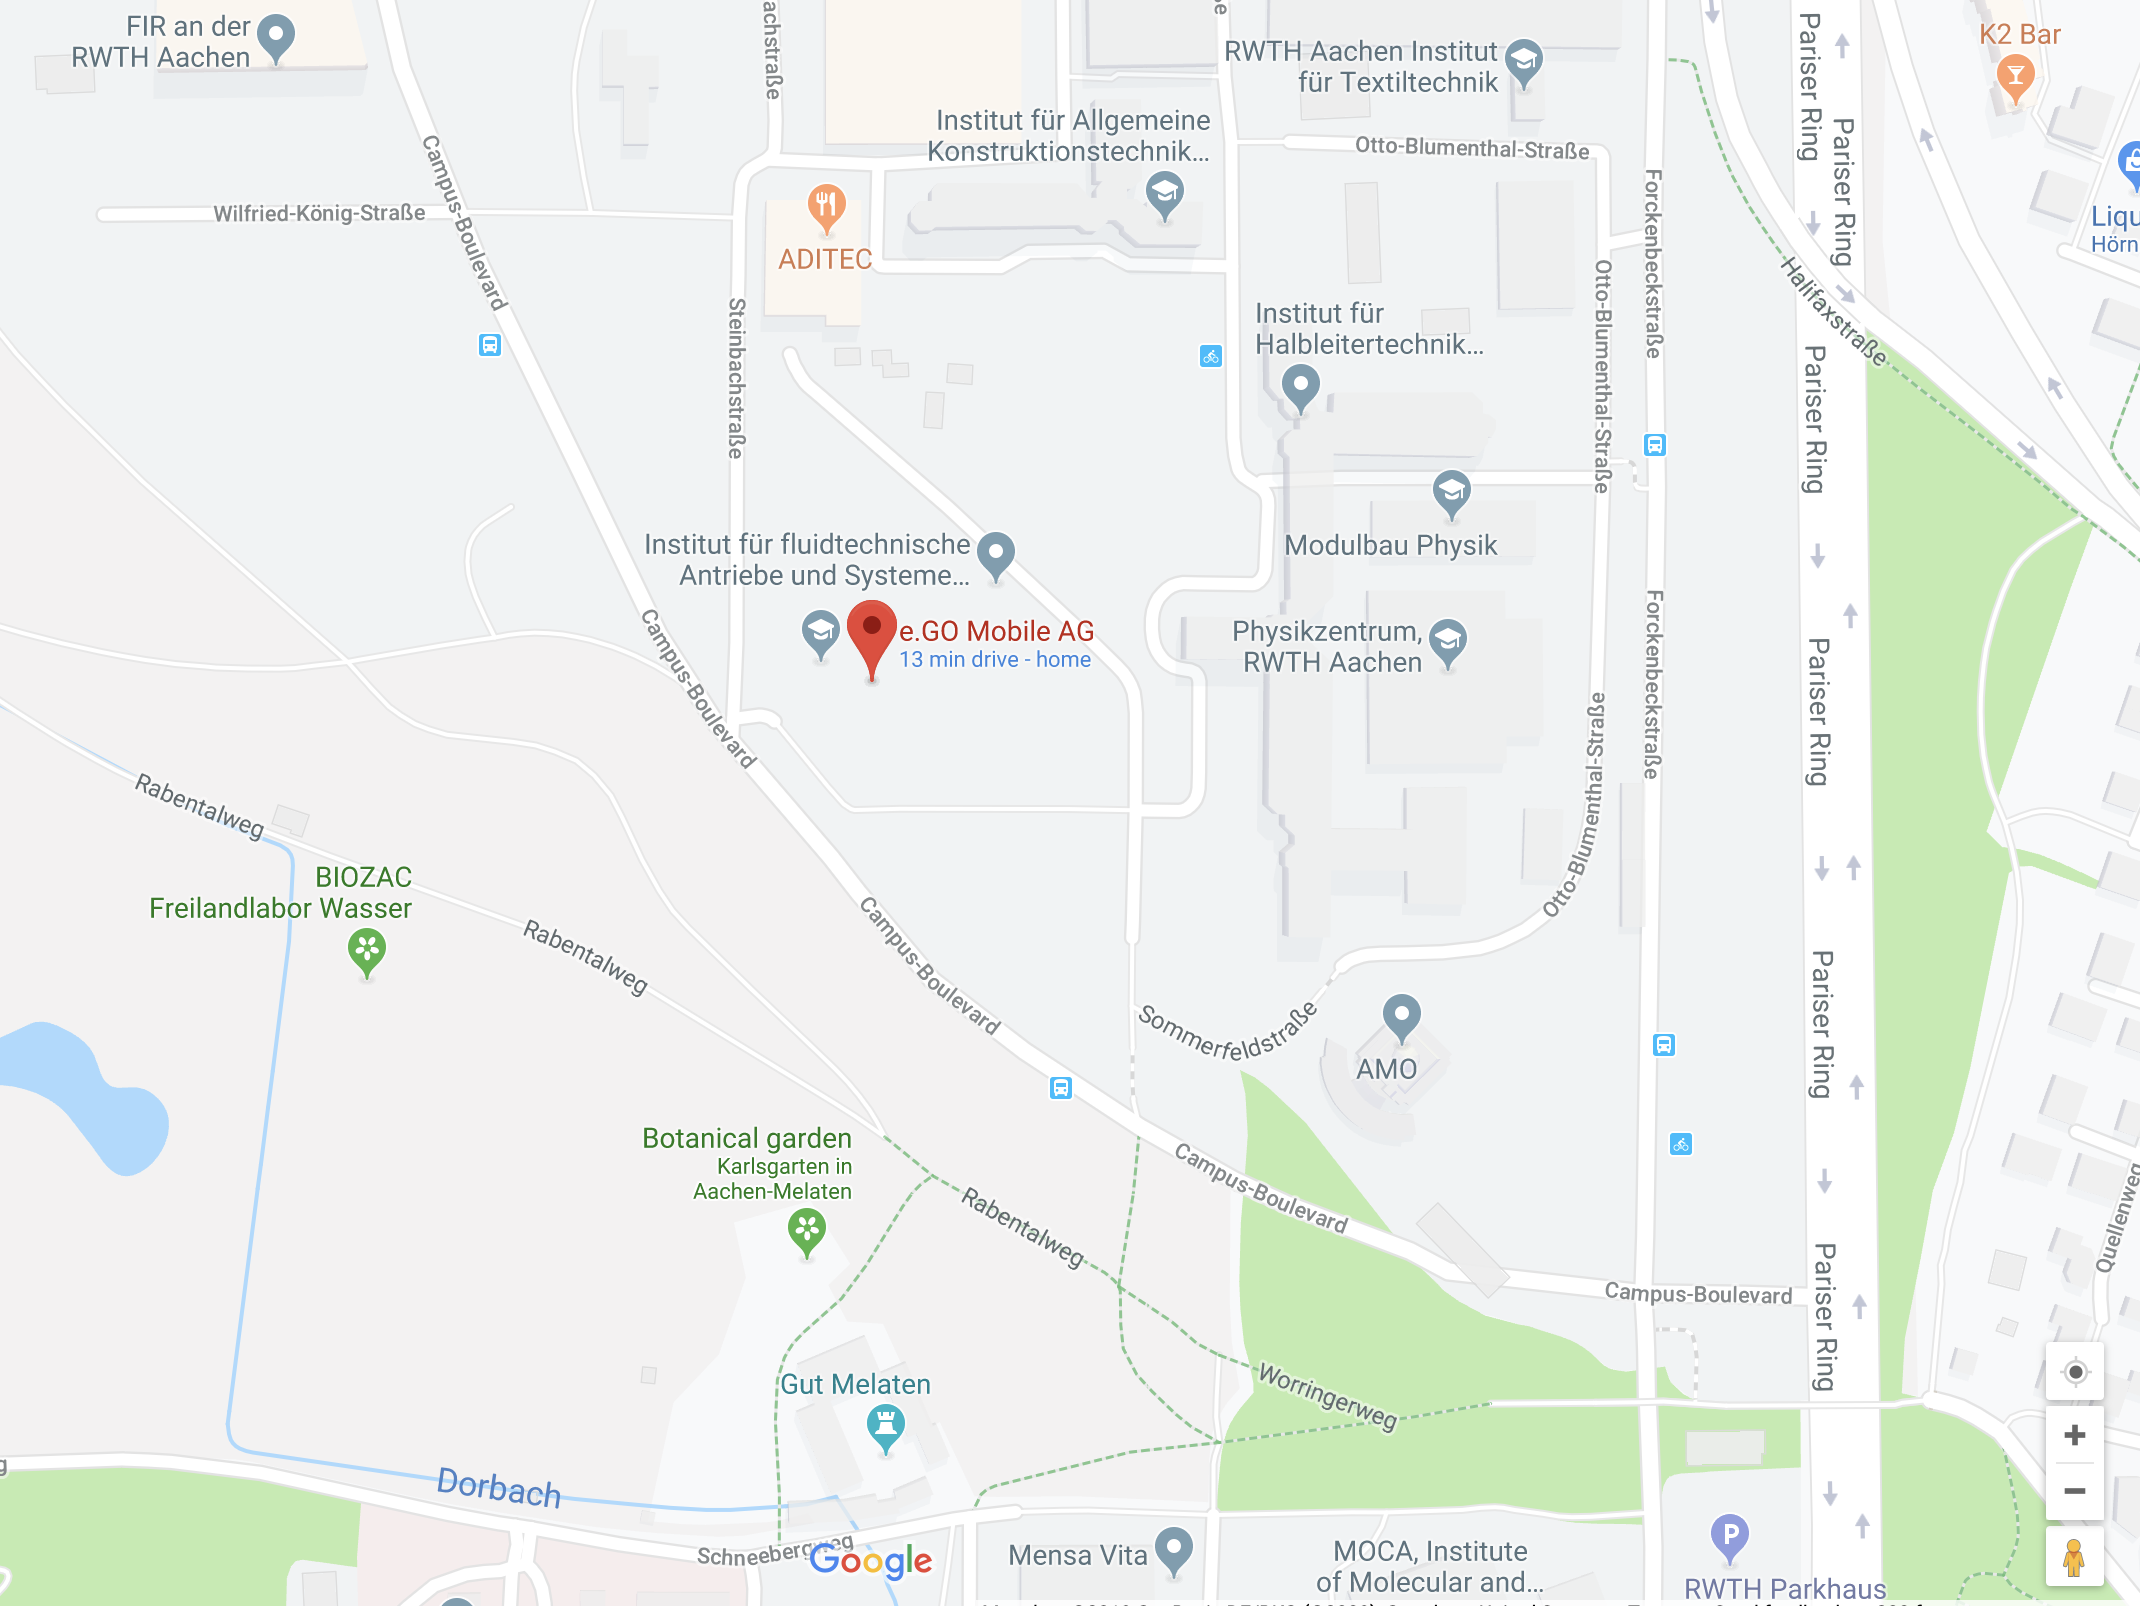
\includegraphics[width=29.72in]{img/google_marker} 

}

\caption{google map with marker}\label{fig:marker}
\end{figure}

\begin{itemize}
\tightlist
\item
  Draw car driving direction
\end{itemize}

\begin{Shaded}
\begin{Highlighting}[]
\NormalTok{knitr}\OperatorTok{::}\KeywordTok{include_graphics}\NormalTok{(}\StringTok{"img/car_direction.png"}\NormalTok{)}
\end{Highlighting}
\end{Shaded}

\begin{figure}

{\centering 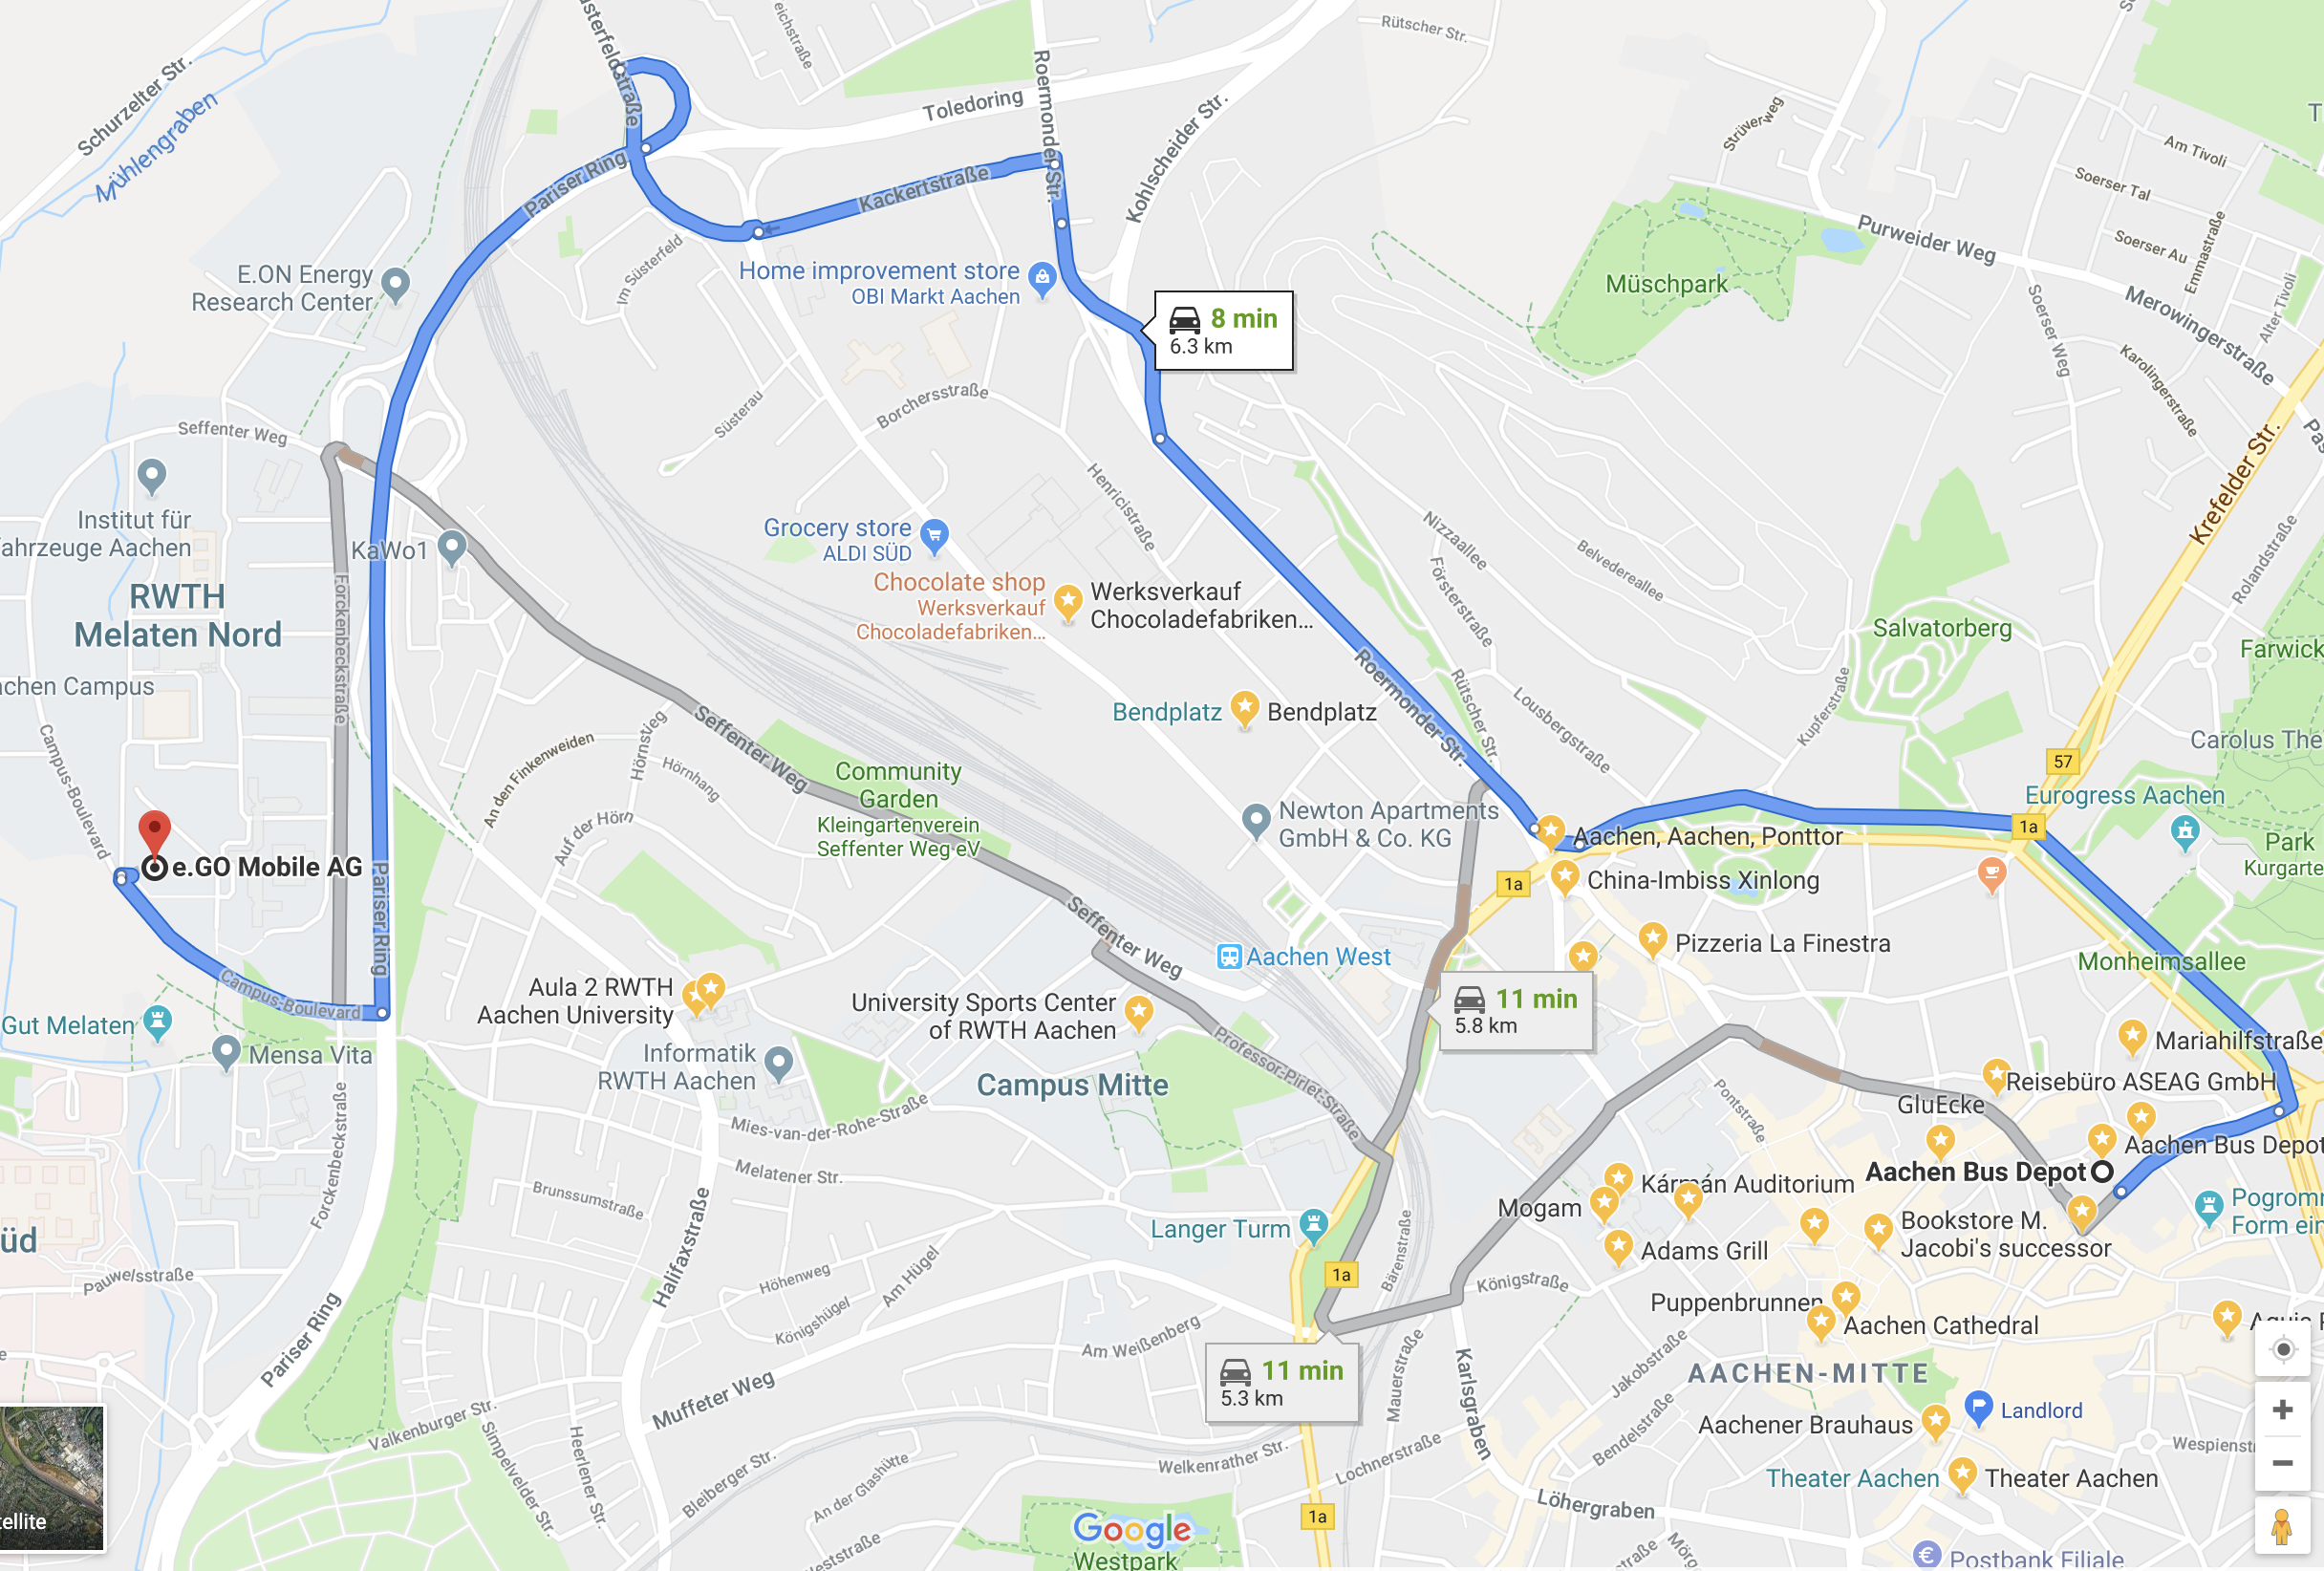
\includegraphics[width=33.78in]{img/car_direction} 

}

\caption{google map with car driving direction}\label{fig:direction}
\end{figure}


\end{document}
